\documentclass[11pt]{article}
\usepackage[a4paper, hmargin={2.8cm, 2.8cm}, vmargin={2.5cm, 2.5cm}]{geometry}
\usepackage{eso-pic} % \AddToShipoutPicture
\usepackage{graphicx} % \includegraphics
\usepackage{listings} % \includegraphics
\usepackage{pgfplots}
\usepackage{hyperref}
\usepackage[utf8]{inputenc}
\usepackage{mdframed}
\usepackage{float}
\usepackage{amsmath}
\usepackage{flafter}
\floatstyle{boxed}
\restylefloat{figure}

\lstset{
  basicstyle=\tiny,
  showspaces=false,
  showstringspaces=false,
  columns=flexible,
  breaklines=true,
  numbers=left
}

%% Change `ku-farve` to `nat-farve` to use SCIENCE's old colors or
%% `natbio-farve` to use SCIENCE's new colors and logo.
\def \ColourPDF {include/ku-farve}

%% Change `ku-en` to `nat-en` to use the `Faculty of Science` header
\def \TitlePDF   {include/ku-en}  % University of Copenhagen

\newcommand{\sasmodels}{\textit{SasModels}}
\newcommand{\sasview}{\textit{SasView}}
\newcommand{\iq}{\texttt{I(q)}}
\newcommand{\foriq}{\texttt{for\_iq}}
\newcommand{\hasiq}{\texttt{has\_iq}}
\newcommand{\futhark}{\texttt{Futhark for SasModels}}
\newcommand{\barheight}{5cm}
\newcommand{\call}{\texttt{\_\_call\_\_}}

\title{
  \vspace{3cm}
  \Huge{\futhark}\\
  \Large{Enhancing performance by rewriting kernels from Python/OpenCL to
    Futhark}
}

\author{
  \Large{Mikkel Storgaard Knudsen}\\
  \texttt{mikkelstorgaard@gmail.com}\\
  \\
  \Large{Supervisor}\\
  Martin Elsman\\
  \texttt{mael@di.ku.dk}
}

\date{
    \today
}

\begin{document}


\AddToShipoutPicture*{\put(0,0){\includegraphics*[viewport=0 0 700 600]{\ColourPDF}}}
\AddToShipoutPicture*{\put(0,602){\includegraphics*[viewport=0 600 700 1600]{\ColourPDF}}}

\AddToShipoutPicture*{\put(0,0){\includegraphics*{\TitlePDF}}}

\clearpage\maketitle
\thispagestyle{empty}
\clearpage
\section*{Abstract}
\sasmodels{} performs small angle scattering calculations for the \sasview{}
modeling suite, by sending its input to a range of calculation models
implemented in Python and OpenCL. 
\\
A Futhark module was written and added to the 
existing \sasmodels{} codebase, to test whether Futhark could outperform the 
already existing model languages used in \sasmodels{}. The Futhark models
were performance tested against a range of the original models.
All following results showed a speed increase of between 200 and 2000\%, 
all without loss of precision.  Speedups were however only apparent at 
unrealistically large input sizes.
\\
Future \sasmodels{} extensions are then suggested, so these speed increases can be 
leveraged in daily \sasview{} usage.

\newpage

\section{Introduction}
\sasview{} is a Small Angle Scattering (SAS) analysis package for the
analysis of 1D and 2D scattering data directly in inverse space.
When \sasview{} is given input data, it performs its analyses by running the
input data through theoretical models provided by the standalone module
\sasmodels{}.
\\\\
\sasmodels{} utilizes a set of kernels, which are implemented
in both Python and OpenCL. However, benchmark
comparisons\cite[sec. 5.3]{array16}
between the parallel algorithm library \textit{Thrust}
(implemented in C++/CUDA), and the array programming language Futhark, shows
that there might be severe speed improvements to gain by running these model
calculations in Futhark, instead of in OpenCL as they are now.\\
\\\\
The goal of \futhark{} is to explore the potential speed gains obtained by
rewriting, and testing the resulting speed improvements of, a subset of the
models in \sasmodels{}.
The subset will be chosen so that there are for each of Python and OpenCL 
one ``simple'' model, and a complex one.
\\\\
If rewriting the models results in a significant\footnote{I.e. a speed increase
  in order of at least 100\%} speedup, it will be reasonable to believe that 
  the rest of the models in \sasmodels{} can be rewritten to obtain a similar
  speedup.

\section{Demonstration of the implementation}
\begin{mdframed}[
  frametitle={Terminology:},
  nobreak=true
  ]
  \futhark{} is spread across multiple parts
  of the \sasmodels{} program. Here is a list of the distinct parts of 
  \sasmodels{} that has been worked with:
  \begin{itemize}
    \item \texttt{kernelfut}: The \sasmodels{} Futhark kernel module that wraps 
    \sasmodels{} input data and sends it to be calculated in the actual Futhark 
    kernel. \texttt{kernelfut} is an alternative to \texttt{kernelpy} and
    \texttt{kernelcl} which are already available in \sasmodels.

    \item Model info files: Every model in \sasmodels{} is defined in a Python 
    model info file, which defines all the model's properties, like the model's
    function itself, and a list of the parameters needed to run the model.
    See figure \ref{fig:dabmodel}

    \item Futhark models: A Futhark model is the model module that contains the
    functions needed to run a given model. See the Futhark line model in figure 
    \ref{fig:linemodel-futhark}
    
    \item The Futhark kernel template, as shown in figure \ref{fig:for-iq}:
    The Futhark kernel template contains the module that takes a Futhark
    model as input, and returns a Futhark kernel that can be called by 
    \texttt{kernelfut}.
    
    \item Futhark kernels: The Python OpenCL library that is produced by 
    compiling the Futhark kernel template with a Futhark model.

    \item \sasmodels{} experiments: A \sasmodels{} experiment is the action of 
    running \sasmodels{} with some input data and one or more models, to get 
    the resulting output data. The output data is the selected models applied
    to the input data.
  \end{itemize}
  
\end{mdframed}

All \sasmodels{} models are described in model info file. These model info 
files has at least two properties:
\begin{itemize}
  \item a function definition \iq{}, which defines scattered intensity 
  of the scattering vector \texttt{q}.

  \item a list \texttt{parameters}, of the parameters that are used in 
  \iq{}. If \iq{} does not take any parameters besides 
  \texttt{q}, the list is left empty.
  In the model info file, the parameters are each defined with their unit name, 
  their default values, their value range, their type of parameter and
  a short text describing what they are.
\end{itemize}

Additionally, the model info file also always contains the short-name, 
the full title, a category, and a mathematical \footnote{a representation 
that compiles to a meaningful mathematical expression if used in a LaTeX math 
environment} string representation of the scattering function.
\\\\
As the scattering function \iq{} and its parameters are the only 
two things that are strictly necessary in a model definition, the developer
has the option to leave the model info defined with just these six properties.
\\\\
\sasmodels{} has built-in default definitions for \texttt{I(qx,qy)} if working
with two-dimensional data, and other functions such as \texttt{form\_volume(q)}
for working with voluminous scatterings.
\\\\
Therefore, it is optional for the developer to define a custom definition
of \texttt{I(qx, qy)} or other default functions.
An example of this can be seen in figure \ref{fig:linemodel}.

\subsection{Defining \iq{} in Python and OpenCL}
A \sasmodels{} \iq{} function can be written in either Python (which will be
executed in a Numpy context at runtime), or it can be written in C, which will
will be inserted into an OpenCL template, so that it can be compiled and 
executed as a kernel in an OpenCL context, preferably on a GPU.
\\\\
A Python \iq{} can be seen in figure \ref{fig:linemodel}, whereas \iq{} for
both DAB 
(figure \ref{fig:dabmodel}) and core\_shell(figure \ref{fig:core_shell})
are written in C.
Notice that the main difference between the models lies in the Iq property.
For Python models, \iq{} is a callable Python function, whilst the C \iq{} is a
 string which is copy-pasted wholesale into the aforementioned OpenCL template.
\\
With \futhark{}, a third way is introduced for using and defining a \sasmodels{} model.

\subsection{Using a Futhark model}
\label{sec:using-futhark}
There is a difference between defining and using a Futhark model.
The \sasview{} user who wishes to use a Futhark model in his or her work does 
not need more than the model info file, and the Futhark kernel.
A Futhark model info file is identical to OpenCL- 
and Python model info files, except for in two properties.
\\\\
As shown in figure \ref{fig:linemodelinfo-futhark}, \iq{} is now a dictionary
with the single flag \texttt{model\_is\_futhark} set to \texttt{True},
and the property \texttt{futhark\_path} points to the location of the Futhark kernel.
\\\\
The user does not need to have the Futhark compiler installed if he merely wants
to use the Futhark kernel: \futhark{} compiles to portable Python libraries which 
has Numpy and Pyopencl as their only dependencies - and as \sasmodels{} has these 
dependencies as well, the user will already have these dependencies sorted out, 
if he has a working installation of \sasview{} or \sasmodels{}.

\subsection{Defining a Futhark model}
\label{sec:defining-futhark-model}
To have a usable Futhark kernel to run in \sasmodels, it is first necessary to
define it as a Futhark program and compile it using \texttt{futhark-pyopencl}.
A Futhark model \textit{m} itself is defined as a parametric Futhark module\footnote{
  A more in-depth explanation of the complete definition of a Futhark module is 
  in sec \ref{sec:generating-futhark}},
which contains an Iq-function, an Iqxy- and a form\_volume function.
It is the model programmers responsibility to fill in all three functions.
\\\\
A simple example is the line module, shown in figure \ref{fig:linemodel-futhark}.
Note that Iqxy is a non-default definition, whilst form\_volume is the default 
definition.

\subsubsection{On the user friendliness of Futhark models}
As apparent from figure \ref{fig:linemodel-futhark}, there are currently two small 
nuisances in Futhark models, compared to equivalent models written in
Python/OpenCL:
\\
With both Python and OpenCL models, the programmer can leave out Iqxy and 
form\_volume so that \sasmodels{} automatically fills in the default definition
for these two functions instead.
\\\\
The Futhark programmer does not have this leisure, but must therefore always
define the two functions. This is boiler plate code, but in the future it could
be solved by compartmentalising the offending functions away in a
parametric library module.
\\\\
Less fixable is it that the programmer must explicitly extract the
Iq function parameters from the list \texttt{local\_values}. This must be done
in the order they appear in the model info parameter list.
\\
Iq functions in Python and OpenCL can be defined with any number of function 
parameters, but Futhark models must adhere to the type declaration of Iq 
(see \texttt{has\_iq} definition in figure \ref{fig:for-iq}), which means that Iq can 
take only two arguments; the scattering vector \texttt{q}, and the list 
\texttt{local\_values} of parameters needed for the scattering.
\\\\
This leads to long preludes to the actual function body Iq function, as in
figure \ref{fig:linemodel-futhark} (line model), or more glaringly like in
figure \ref{fig:core_shell} (core shell model).

\subsection{Generating Futhark models using parametric modules and a header}
\label{sec:generating-futhark}
As mentioned in sec. \ref{sec:defining-futhark-model}, the Futhark model developer
does only need to define three functions to be able to compile a working 
\sasmodels{} Futhark model.
However, those three functions are merely used by a parametric Futhark module 
\foriq{}, which takes care of the actual execution of the 
Futhark kernel.
Let's go through the actual implementation of the Futhark models.

\subsubsection{line\_futhark.fut (a Futhark model)}
\label{sec:line-fut}

\begin{figure}
  \lstinputlisting[]{../sasmodels/sasmodels/models/futharks/line_futhark.fut}
  \caption{The complete definition of the line model implemented in Futhark.}
  \label{fig:linemodel-futhark-full}
\end{figure}

Several things are happening in line\_futhark.fut besides (figure
\ref{fig:linemodel-futhark-full}), besides the definition of the line Iq function.
\\
\\
\texttt{module line} takes either single- or double precision floats as a
parameter, and then assigns the type alias \texttt{dtype} to the type of the
input parameter. This means that we can use \texttt{dtype} in the type
declarations throughout the module, and define the module for floats in general,
instead of maybe having to define linef64- and linef32 modules.
\\\\
Then, two kernels (one for each of f32 and f64) are initialised by giving
the parametric module \texttt{for\_iq} the line module and a data type 
as parameters, returning \texttt{kernel\_float32} and \texttt{kernel\_float64}.
\\
Given these two modules, we can finally define four entry points into the
finished model. These are the four entry points that can be called by 
\sasmodels{} whenever a \sasmodels{} experiment needs to execute calculations 
in a Futhark kernel.
Each of the entry points are simply passing on their call parameters to the 
\texttt{run\_kernel} functions defined in the \texttt{for\_iq} module.
Everything after the module line definition is boilerplate code, and could
possibly be defined in a more elegant way in a later revision, but currently, it 
is a necessary part of every Futhark model.
\\\\
Other models, such as core shell, imports libraries which are then
available in the Iq function.

\subsubsection{header/for\_iq.fut (the Futhark kernel template)}
The file \texttt{for\_iq.fut} contains the module type declaration for the \hasiq{} module,
 and it contains the definition of the parametric \foriq{} module. 
\\
The type declaration \hasiq{} ensures, that any model module that is
used as a parameter for the \foriq{} module defines at least the functions
Iq, Iqxy and form\_volume, as these functions are necessary for the definition
of the Futhark kernel.
\\\\
Next, we have the actual definition of the module \foriq{}, which takes two parameters (a parametric Futhark model), and a real type to instantiate it with.
It then instantiates the model with the real type, making the finished Iq module
\texttt{Iq} available throughout the rest of the kernel.
\\
Then finally, it uses the Iq module to define the two functions 
\texttt{run\_kernel}, and \texttt{run\_kernel\_2d}, which defines the actual 
\sasmodels{} computation procedure with the scattering functions injected by 
the Iq module.

\begin{figure}
  \lstinputlisting[]{../sasmodels/sasmodels/models/futharks/header/for_iq.fut}
  \caption{The Futhark template that is used by the individual models. Notice
    that this template is not copied, but appears only once in the system - it
    is shared between the Futhark models.}
  \label{fig:for-iq}
\end{figure}

\subsubsection{Why not implement Futhark models as model info strings 
instead of standalone modules?}
OpenCL kernels are generated by copy/pasting the desired \iq function body
into a template, and then compiling the resulting source code.
This happens at runtime in \sasmodels, which means that the kernels aren't
 actually compiled until right before \sasmodels{} needs them.
\\\\
Futhark models eschews this design and opts instead to separate code generation
and model usage completely.
It would be simple to copy the design of the OpenCL kernels, and compile Futhark
kernels at \sasmodels{} runtime, but this design was cast aside in favour of the
design described in sec \ref{sec:generating-futhark}.
\\
There are three reasons for this decision:
\begin{enumerate}
  \item Removing code generation from runtime unequivocally decreases the time
  it takes to run a \sasmodels{} calculation. Although time taken by code 
  generation is not covered by \sasmodels' built-in benchmark modules, it should
  be obvious that a program that merely executes a kernel computation has a 
  shorter runtime than a program that has to compile the kernel before it
  executes the kernel computation.
  
  \item Compiling a kernel just in time brings the risk of encountering 
  Futhark compilation errors at \sasmodels{} runtime. 
  It is arguably a user experience nightmare to encounter compilation errors at 
  runtime, which is why Futhark models keeps compilation separate from runtime.
  
  \item Compiling Futhark models down to self-contained\footnote{depending only 
  on Numpy and Pyopencl} Python libraries means that Futhark models are 
  completely portable, and as such can be used by any \sasmodels{} or \sasview{} 
  user, without them needing to have a Futhark compiler installed on their 
  workstations.
\end{enumerate}

\section{Adding \texttt{kernelfut} to \sasmodels}
The following process happens when running a \sasmodels{} experiment through the
built-in comparison module:
\begin{figure}
  
\begin{enumerate}
  \item The experiment parameters\footnote{choice(s) of model, number of 
  evaluations, sample size, number type and so on} for the experiment are used
  to create a ParameterTable.
  
  \item The ParameterTable is used to load (or generate) a set of input data for
   the kernel.

  \item The ParameterTable is used to initialize a \sasmodels{} kernel using the
  desired model. In case of OpenCL and Futhark kernels, the input data is 
  buffered to the OpenCL context already at this point. This is done to leave
  as much buffering out of the time measurements of \sasmodels{} as possible.
  
  \item \sasmodels{} packs the model and the data in a DirectModel wrapper object.

  \item The DirectModel is run the desired number of times in \sasmodels,
  and finally returns the model output, the average running time, and the
  output difference between the models that have been compared. 
\end{enumerate}
\end{figure}

To design \texttt{kernelfut}, it was first necessary to ape the 
\sasmodels{} calculation loop as a Futhark function. 
I chose to replicate \texttt{kernelpy}'s \texttt{\_loops(...)} function in 
Futhark, as it is fairly simple to rewrite the Python code in Futhark.
\texttt{\_loops()} is shown in figure \ref{fig:kernelpy_loop}, and the
comparable Futhark function in figure \ref{fig:kernelfut_loop}.
\\\\
Second, it was necessary to implement a bridge between \sasmodels{} and the 
precompiled Futhark kernels. 
When \sasmodels{} wants to use a Futhark kernel for it's calculations, 
it must dynamically import the kernel during the initialisation of the FutKernel
object. Figure \ref{fig:retrieving-futhark-class} shows how FutKernel uses
the path and model name from the model info file, to load and initialize the
model class that is available in the compiled Futhark kernel.
\\\\
After the Futhark kernel has been initialised and made available to FutKernel,
we can retrieve the kernel's OpenCL queue, and buffer our input data onto the 
OpenCL device immediately, so we don't have to spend time doing this during 
kernel execution itself.
Doing this reduces the Futhark overhead during kernel execution by between
200 and 800 milliseconds.
\\\\
Finally, the FutKernel's \texttt{\_form} attribute is set. \texttt{\_form} is the entry point from
the Futhark kernel, as seen in figure \ref{fig:linemodel-futhark-full}.

%% what is form??
\begin{figure}
  \lstinputlisting[linerange={30-32, 55-56, 74-82, 121-126}, language=Python]{../sasmodels/sasmodels/kernelfut.py}
  \caption{Injecting the precompiled Futhark kernel in the FutKernel object}
  \label{fig:retrieving-futhark-class}
\end{figure}


\begin{figure}
  \lstinputlisting[linerange={128-140}, language=Python]{../sasmodels/sasmodels/kernelfut.py}
  \caption{Buffering the input data to the Futhark kernel's queue}
  \label{fig:buffering-kernelfut}
\end{figure}

Like with \texttt{kernelcl} and \texttt{kernelpy}, FutKernel must also implement
\call{} so that DirectModel can call the model and perform the
calculations.
This has been done by writing a simplified version of the OpenCL kernel's 
\call{} function. 
\\\\
As seen in figure \ref{fig:kernelfut_call} and figure \ref{fig:kernelcl_call},
the primary task of the call function is to pack an array of arguments, and
pass them on as arguments for a kernel.
As \call{} must return a numpy array, the get() function is called at the end
of the Futhark kernel call, to convert the output OpenCL Array into a 
numpy array.
\\\\
Note that kernelfut does not have the evaluation loop that kernelcl has.
The loop still exists, but has been moved inside of the Futhark template 
instead (see figure \ref{fig:for-iq}).

\section{Method}
\sasmodels{} contains a comparison module called \texttt{compare.py}, which
lets the user run different calculations on the same dataset.
This module has been the basis of all my performance tests, and indeed also
the module that has let me design Futhark models in the first place.
\\\\
The development of Futhark for \sasmodels{} has been largely test-driven.
For any given already existing model in the \sasmodels{} catalogue that I have
wished to implement in Futhark, I have started out by defining an equivalent
model written in Futhark, and then used the comparison module to compare the
 runs of the original model versus the Futhark implementation.
\\\\
The comparison module displays the average execution time of each of the models,
which lets me track exactly how much faster (or slower) the Futhark model has
been running, compared to the original implementation.
\\\\
Furthermore, and ultimately most important, the comparison module also
revealed the difference in results between the two models. 
As I have limited knowledge about the field of Small Angle Scatterings, 
the only option for me regarding correctness of the models has been to take
the results of the already existing models as the "correct" results of the
computations. Consequently, any difference between my Futhark results and the
original results has been direct indicators of faulty implementations or bugs
somewhere in my work.
Therefore, I have been developing and debugging my solution by repeatedly
comparing it's results to that of the original implementation.
\\\\
Conversely, I have chosen to accept test runs with exactly no difference
between the original and the Futhark implementation, as indicators of a
correct implementation. 
Test runs with thousands of data points defined as double-precision
with more than ten decimal points have still resulted in a total difference of
zero\footnote{see sec. \ref{sec:correctness}} between the models.
\\
This is what I base my assertion of a correctness on, as even the smallest 
mistakes along the calculations would surely have resulted in a very significant
accumulated error in the final results.
\\\\
The test driven development has also lead to some of the biggest performance
optimizations in my design of kernelfut.py.
In the example, the initial tests showed that the Futhark kernels were unreasonably
slower than the already existing kernels. After some investigation I found
that this was because the original implementation buffered the input data in the
OpenCL context long time before the actual kernel was called in Python, whereas
the first versions of the Futhark kernel buffered the input data in the OpenCL
context as part of the \texttt{run\_kernel} function call.

\section{Performance results}
\label{sec:performance}
\subsection{Futhark vs. Python performance}
I have tested Futhark vs. Python performance on two different models; 
the \texttt{line} model and the \texttt{broad\_peak} model.

\subsubsection{\texttt{line} model}
The \iq function for the line model is defined as $I(q) = A + B*q$, which is
equivalent to one of the most basic high school math functions, $f(x) = ax + b$.

\begin{figure}
    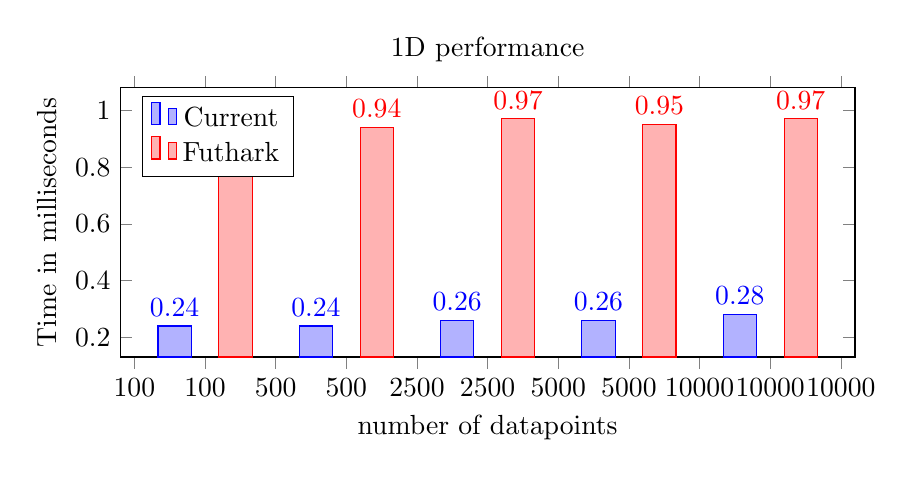
\begin{tikzpicture}
      \begin{axis}[
        title={1D performance},
        xlabel={number of datapoints},
        ylabel={Time in milliseconds},
        width=0.9\textwidth,
        height=\barheight,
        symbolic x coords={100,500,2500,5000,10000},
        bar width=9pt,
        enlargelimits=0.15,
        ybar=10pt,% configures ‘bar shift’
        bar width=12pt,
        nodes near coords,
        legend style={legend pos=north west}
      ]
      \addplot plot coordinates {(100, 0.24 ) (500, 0.24 ) (2500, 0.26 ) (5000, 0.26 ) (10000, 0.28 )};
      \addplot plot coordinates {(100, 0.93 ) (500, 0.94 ) (2500, 0.97 ) (5000, 0.95 ) (10000, 0.97 )};
      \legend{Current, Futhark}
      \end{axis}
    \end{tikzpicture}
    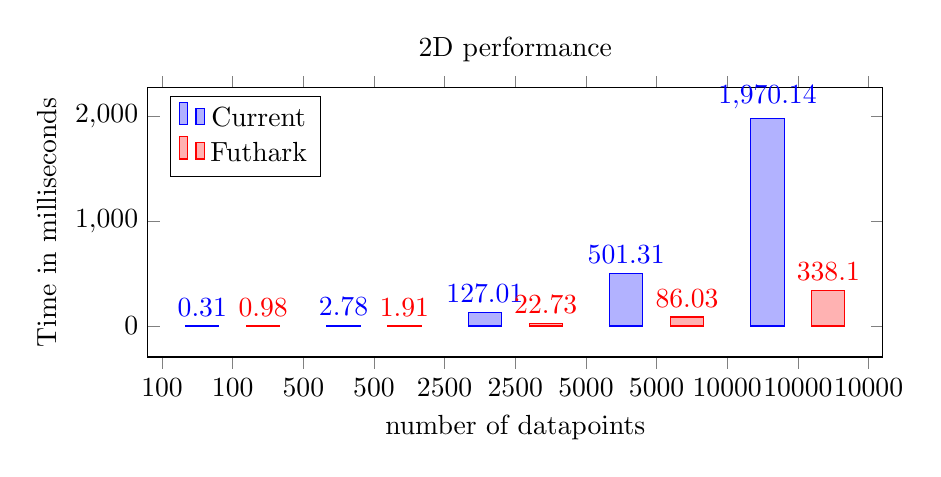
\begin{tikzpicture}
      \begin{axis}[
        title={2D performance},
        xlabel={number of datapoints},
        ylabel={Time in milliseconds},
        width=0.9\textwidth,
        height=\barheight,
        symbolic x coords={100,500,2500,5000,10000},
        bar width=9pt,
        enlargelimits=0.15,
        ybar=10pt,% configures ‘bar shift’
        bar width=12pt,
        nodes near coords,
        legend style={legend pos=north west}
      ]
      \addplot plot coordinates {(100, 0.31 ) (500, 2.78 ) (2500, 127.01 ) (5000, 501.31 ) (10000, 1970.14 )};
      \addplot plot coordinates {(100, 0.98 ) (500, 1.91 ) (2500, 22.73 ) (5000, 86.03 ) (10000, 338.10 )};

      \legend{Current, Futhark}

      \end{axis}
    \end{tikzpicture}
    \caption{Comparison between Python and Futhark performance for simple model}
    \label{fig:line-graph}
\end{figure}

In figure \ref{fig:line-graph} we see that for one dimensional calculations,
both implementations keep a steady execution time. Futhark is consistently 
slower, but that can be explained by the overhead of launching the Futhark kernels.
\\\\
More interesting is it to look at the execution time of the 2D version of the 
experiment. For all \sasmodels{} 2D experiments, we are not just calculating \iq
for each q, but actually $\sum_{q \in Q} \sum_{q \in Q} Iq(q_x, q_y)$.
So if we have a q vector of $n$ elements, we need to perform $n^2$ calculations.
\\\\
We see in the figure, that Futhark at $10000^2$ datapoints now greatly outperforms
the Python model.

\subsubsection{\texttt{broad\_peak} model}
\texttt{broad\_peak} is quite different than the line model from before (see
figure \ref{fig:broadpeakmodel}). Its \iq
function is defined as 
$I(q) = \frac{A}{q^n} + \frac{C}{1 + (|q - q_0|\xi)^m} + B$.\footnote{see \url{http://www.sasview.org/docs/user/models/broad_peak.html}}

\begin{figure}
      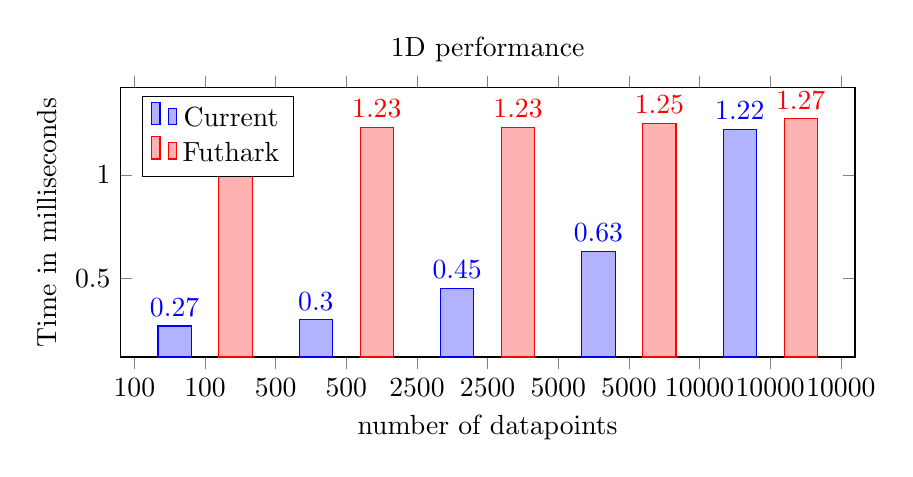
\begin{tikzpicture}
      \begin{axis}[
        title={1D performance},
        xlabel={number of datapoints},
        ylabel={Time in milliseconds},
        width=0.9\textwidth,
        height=\barheight,
        symbolic x coords={100,500,2500,5000,10000},
        bar width=9pt,
        enlargelimits=0.15,
        ybar=10pt,% configures ‘bar shift’
        bar width=12pt,
        nodes near coords,
        legend style={legend pos=north west}
      ]
      \addplot plot coordinates {(100,0.27) (500,0.30) (2500,0.45) (5000,0.63) (10000,1.22)};
      \addplot plot coordinates {(100,1.22) (500,1.23) (2500,1.23) (5000,1.25) (10000,1.27)};

      \legend{Current, Futhark}
      \end{axis}
    \end{tikzpicture}
    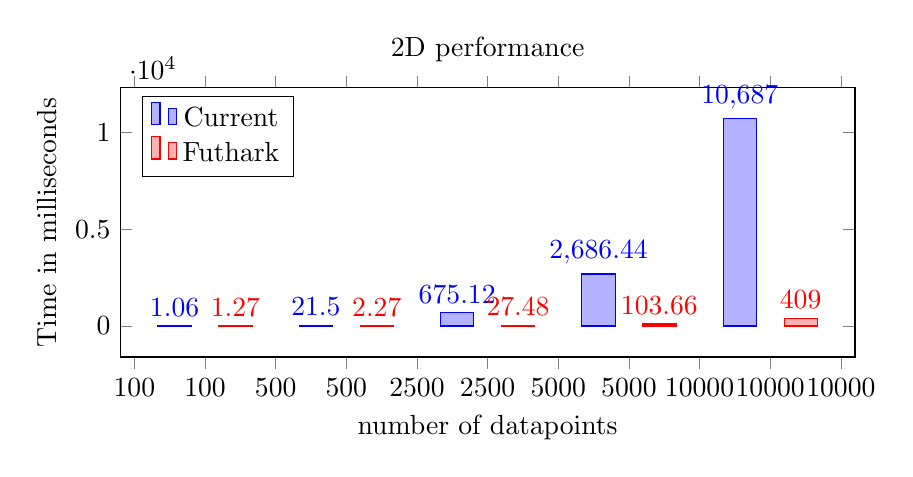
\begin{tikzpicture}
      \begin{axis}[
        title={2D performance},
        xlabel={number of datapoints},
        ylabel={Time in milliseconds},
        width=0.9\textwidth,
        height=\barheight,
        symbolic x coords={100,500,2500,5000,10000},
        bar width=9pt,
        enlargelimits=0.15,
        ybar=10pt,% configures ‘bar shift’
        bar width=12pt,
        nodes near coords,
        legend style={legend pos=north west}
      ]
      \addplot plot coordinates {(100,1.06 ) (500,21.50 ) (2500,675.12) (5000,2686.44 ) (10000,10687)};
      \addplot plot coordinates {(100,1.27 ) (500,2.27 ) (2500,27.48) (5000,103.66 ) (10000,409)};

      \legend{Current, Futhark}

      \end{axis}
    \end{tikzpicture}
    \caption{Comparison between Python and Futhark performance for complex model}
    \label{fig:broad-peak-graph}
\end{figure}

In figure \ref{fig:line-graph} we see that for one dimensional calculations,
both implementations keep a steady execution time. Futhark is consistently 
slower, but, again, that can be explained by the overhead of launching the Futhark kernels.
\\\\
More interesting is it to look at the execution time of the 2D version of the 
experiment. As explained earlier, all \sasmodels{} 2D experiments are not just calculating \iq
for each q, but actually $\sum_{q \in Q} \sum_{q \in Q} Iq(q_x, q_y)$.
So if we have $n$ elements in $Q$ , we need to perform $n^2$ calculations.
\\\\
We see in the figure, that Futhark at $10000^2$ datapoints now greatly outperforms
the Python model.

\begin{mdframed}[
  frametitle={Why does Futhark perform faster than Python?},
  nobreak=true
  ]
These comparisons are between Python/Numpy- and Futhark models.
Although Numpy can execute both of the models as vectorized calculations, 
it is still vastly outperformed by Futhark, which can run hundreds of threads 
simultaneously on the GPU. In comparison, Numpy runs on the CPU, which rarely 
runs more than 10-20 threads simultaneously.
\\
For models like broad\_peak, Futhark gains a significant speedup by 
hoisting\cite[sec 2.3]{pldi17} the allocation of variables 
(figure \ref{fig:broadpeakmodel_futhark}) outside of
the function call, so they are allocated as constants in the \foriq{} 
\texttt{run\_kernel} function, right before mapping Iq.Iq over the q input.
\\\\
Hoisting is not uncommon for compilers to do at all, but it does make a 
difference for \sasmodels{}.
The compiler moves the number of variable allocations from
$O(\text{length of q vector } \cdot \text{number of parameters})$ to 
$O(\text{number of parameters})$.
\end{mdframed}

\subsection{Futhark vs. OpenCL performance}
\subsubsection{The \texttt{DAB} model}
The \texttt{DAB} model (figure \ref{fig:dabmodel}) is relatively simple, as it is described as $I(q) = \frac{L^3}{1 + (qL)^2}$,
requiring us to work with just one single variable.
  \begin{figure}
    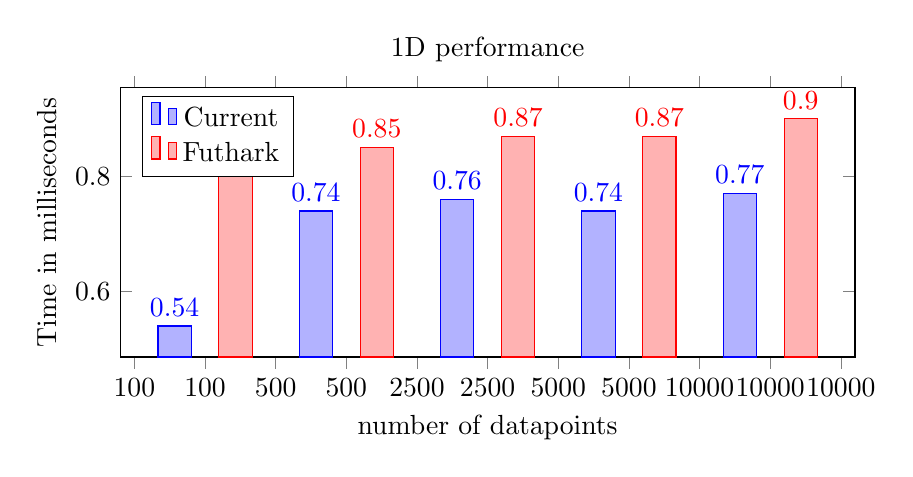
\begin{tikzpicture}
      \begin{axis}[
        title={1D performance},
        xlabel={number of datapoints},
        ylabel={Time in milliseconds},
        width=0.9\textwidth,
        height=\barheight,
        symbolic x coords={100,500,2500,5000,10000},
        bar width=9pt,
        enlargelimits=0.15,
        ybar=10pt,% configures ‘bar shift’
        bar width=12pt,
        nodes near coords,
        legend style={legend pos=north west}
      ]
      \addplot plot coordinates {(100, 0.54 ) (500, 0.74 ) (2500, 0.76 ) (5000, 0.74 ) (10000, 0.77 )};
      \addplot plot coordinates {(100, 0.86 ) (500, 0.85 ) (2500, 0.87 ) (5000, 0.87 ) (10000, 0.90 )};

      \legend{Current, Futhark}

      \end{axis}
    \end{tikzpicture}
    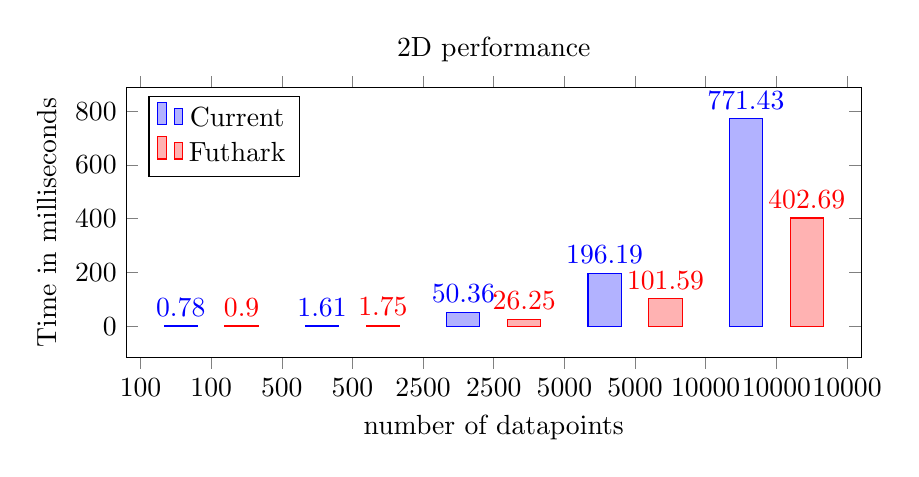
\begin{tikzpicture}
      \begin{axis}[
        title={2D performance},
        xlabel={number of datapoints},
        ylabel={Time in milliseconds},
        width=0.9\textwidth,
        height=\barheight,
        symbolic x coords={100,500,2500,5000,10000},
        bar width=9pt,
        enlargelimits=0.15,
        ybar=10pt,% configures ‘bar shift’
        bar width=12pt,
        nodes near coords,
        legend style={legend pos=north west}
      ]
      \addplot plot coordinates {(100, 0.78 ) (500, 1.61 ) (2500, 50.36 ) (5000, 196.19 ) (10000, 771.43 )};
      \addplot plot coordinates {(100, 0.90 ) (500, 1.75 ) (2500, 26.25 ) (5000, 101.59 ) (10000, 402.69 )};

      \legend{Current, Futhark}

      \end{axis}
    \end{tikzpicture}
    \caption{Comparison between OpenCL and Futhark performance for simple model}
    \label{fig:dab-graph}
  \end{figure}


\subsubsection{The \texttt{Core Shell Parallelepiped} model}
The \texttt{Core Shell Parallelepiped} model is by far one of the most complex models
in \sasmodels' catalogue (figure \ref{fig:core_shell}). 
With its more than ten parameters and its nested loops, it is 
a candidate model for the Futhark compiler to attempt to optimize.
  \begin{figure}
    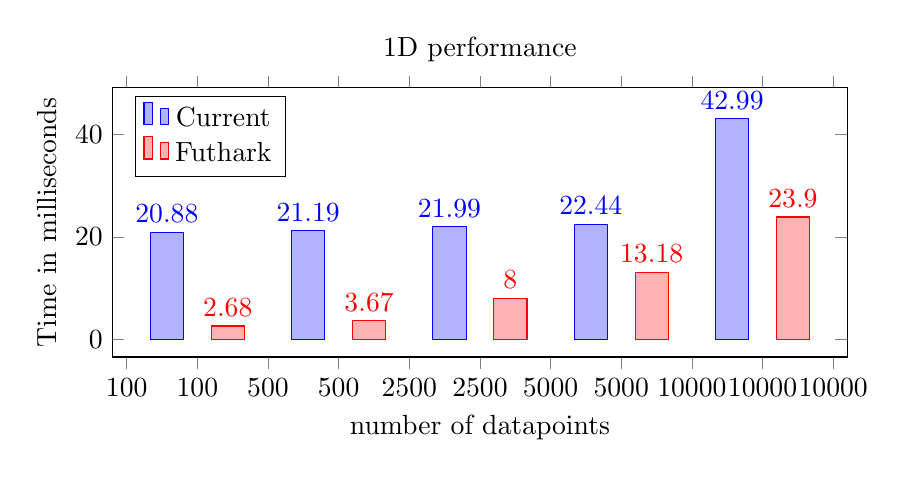
\begin{tikzpicture}
      \begin{axis}[
        title={1D performance},
        xlabel={number of datapoints},
        ylabel={Time in milliseconds},
        width=0.9\textwidth,
        height=\barheight,
        symbolic x coords={100,500,2500,5000,10000},
        bar width=9pt,
        enlargelimits=0.15,
        ybar=10pt,% configures ‘bar shift’
        bar width=12pt,
        nodes near coords,
        legend style={legend pos=north west}
      ]
      \addplot plot coordinates {(100, 20.88 ) (500, 21.19 ) (2500, 21.99) (5000, 22.44 ) (10000, 42.99)};
      \addplot plot coordinates {(100, 2.68 ) (500, 3.67 ) (2500, 8.00 ) (5000, 13.18 ) (10000,23.90 )};

      \legend{Current, Futhark}

      \end{axis}
    \end{tikzpicture}
    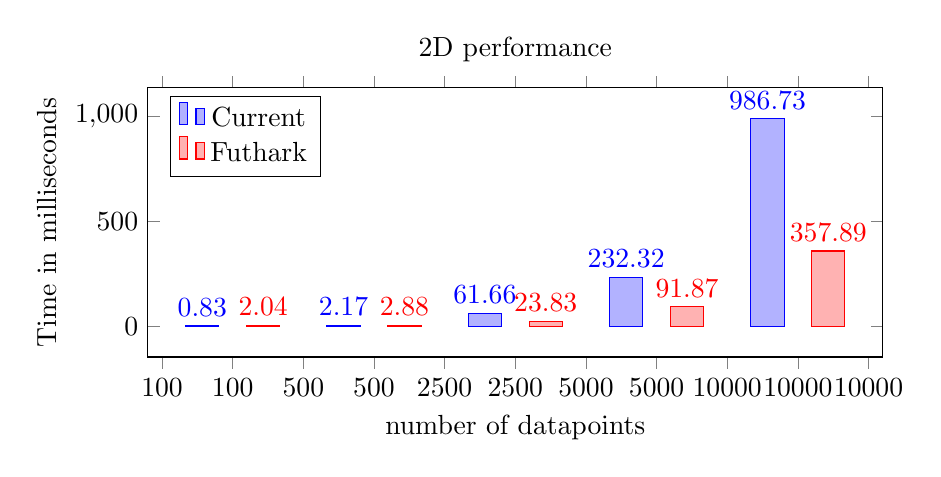
\begin{tikzpicture}
      \begin{axis}[
        title={2D performance},
        xlabel={number of datapoints},
        ylabel={Time in milliseconds},
        width=0.9\textwidth,
        height=\barheight,
        symbolic x coords={100,500,2500,5000,10000},
        bar width=9pt,
        enlargelimits=0.15,
        ybar=10pt,% configures ‘bar shift’
        bar width=12pt,
        nodes near coords,
        legend style={legend pos=north west}
      ]
      \addplot plot coordinates {(100, 0.83 ) (500, 2.17 ) (2500, 61.66 ) (5000, 232.32 ) (10000, 986.73 )};
      \addplot plot coordinates {(100, 2.04 ) (500, 2.88 ) (2500, 23.83 ) (5000, 91.87 ) (10000, 357.89 )};

      \legend{Current, Futhark}

      \end{axis}
    \end{tikzpicture}
    \caption{Comparison between OpenCL and Futhark performance for complex model}
    \label{fig:core-shell-graph}
  \end{figure}

\begin{mdframed}[
    frametitle={Why does Futhark perform faster than OpenCL?},
    nobreak=true]

While it was expected to see Futhark outperform the strictly CPU based 
computations performed by Numpy in the Python models, it was more uncertain
how much (or even whether) Futhark would outperform OpenCL.
\\\\
However, data shows that Futhark does perform better. The increased performance 
in figure \ref{fig:dab-graph} is not really significant until we reach very high
n, which can be attributed to the simplicity of the model.
\\
With such simple models, there are not many things that Futhark can do smarter 
than the normal OpenCL compiler, besides the gains that are possible from
the aforementioned hoisting.
\\\\
However, when we work with the rewritten core shell parallelepiped, we see huge
speedups even at n=100. This speedup comes from the Futhark compiler's 
nested \texttt{map} optimizations: the Iq function is mapped
over the array of q values, and the Iq function body is mainly a nested 
map-map-reduce-reduce, which makes the final nested function a 
map-map-map-reduce-reduce. 
\\
As this construct can be flattened and parallelised\cite[sec. 5]{pldi17}, 
we are can split our workload into many more tasks than the original OpenCL 
implementation, which only has nq tasks. However, every single of these tasks
consists of complex for-loop nests, and plenty of variable assignments.
\\\\
Furthermore, the Futhark compiler takes care to ensure that the calculations 
over the Gauss arrays and q values are coalesced, so we are given 
efficient memory access.
\\
For the original OpenCL implementation, we risk that different kernels are
accessing memory locations that are physically far apart, so that the GPU
has to handle the memory accesses individually, instead of being able to 
combine them.
\end{mdframed}

\subsection{Correctness of Futhark results}
\label{sec:correctness}
There has been one small issue with the correctness of the Futhark models.
As the Futhark models are generic by design, and instantiated with the 
programmer's floating point type of choice, we can run the Futhark kernels
with any precision we want.
\\\\
However, some of the original model implementations \sasmodels{} have Iq functions that are 
hardcoded to use double precision floats in places, and even sometimes mixes
doubles and singles. 
As these models plays fast and loose with the precision type, the Futhark models
will inevitably end up showing some total difference between it's results and 
the results from the built in functions.
\\\\
However, several \sasview{} users have assured me, that it is not really a 
problem. The worst examples of these differences has been accumulated errors of
between 10e-6 and 10e-7, which is well within the error range accepted by 
the \sasview{} users.
\section{Discussion, future work}
\label{sec:discussion}
The performance tests in sec. \ref{sec:performance} unequivocally shows, that
there are speedups to gain by running Futhark kernels in favor of Python or
OpenCL kernels.
In general, Futhark starts surpassing the performance of competing kernels, when
sample sizes rise above n=INDSÆT N. However, these gains are currently
irrelevant for the most \sasview{} use cases, as almost all
experiments are carried out on sample sizes of between 100-500.
However, meetings with external project owner Wojciech Potrzebowski lead to the
suggestion that simple bundling of \sasview{} experiments would enable us
to leverage the Futhark speed improvements directly.
\\\\
For example, one could imagine running an experiment that continuously sends
sensor data for processing in \sasview{} / \sasmodels.
Instead of running an experiment for each sample\footnote{of size n=100-500}
from the stream, one could let \sasmodels{} bundle these input samples in packages
of 10-50 samples
instead, and calculate these collectively to leverage the speedups that are
apparent on Futhark calculations on samples of larger sizes.
\\\\
Please note, that sample sizes might have an upper bound, depending on the
memory available on the workstations running the experiments.

\subsection{Finding the best match in \sasview}
\label{sec:best-match}
In addition to bundling input data, Wojciech also suggested that the Futhark
speedups could be used to implement faster best-match-finding for \sasview
experiments.
\\\\
Among other things, \sasview{} is used to test multiple models against a data set,
to find out which of the models that actually fits the data most closely.
Currently this is not done in an efficient manner.
Therefore, it would be interesting to implement a way of running multiple models
on the same data set in parallel.
And given the current Futhark vs. OpenCL results, the implementation should
be pursued in Futhark, as it has already been shown to be advantageous
(compared to Open CL).


\subsection{Usability of Futhark models}
It is relevant to discuss how useful Futhark models are to the \sasview{} user
groups. For the users who merely wants to use the models, it is not necessary
to understand the implementation itself at all, as the user facing part of
the model is just the model info file, which is just the same as the model infos
for Python and OpenCL models (see sec. \ref{sec:using-futhark}).
\\\\
However, for the model developer, it is now also necessary to have at least a
rudimentary understanding of functional programming.
In example, developers will have to learn how to use maps in Futhark in
places where they would usually use loops in Python and C.
\\\\
Furthermore, the current solution requires severe amounts of boilerplate code to
be included in the Futhark model file.
This boilerplate is caused by the usage of Futhark's module system, and
therefore not strictly part of defining the \iq function of a model.
For instance, the boilerplate might become a distraction for the model developer, so
there might be a smaller educational challenge to solve here as well.
\\\\
\subsection{Why should \sasmodels{} developers use Futhark?}
Currently, large scale data processing can be an unpleasant endeavor in
\sasmodels{}, as some of the models (especially the Python based ones) have
got runtimes that makes \sasview{} itself slow and irksome to work with.
\\
With Futhark models, the developers are assured that their models are being
optimized by a compiler automatically - at least as long as they choose to
follow sound functional programming patterns.\\
All in all, \futhark{} could simply lead to a faster (and thereby nicer)
experience for \sasview{} users.
\\\\
That Futhark models must be compiled before being available to \sasmodels{} at
all, also aides the \sasmodels{} developer in designing his models. With the
exception of out-of-bounds errors stemming from bad indexes into the parameters
list, the Futhark type checker ensures that mistakes are discovered on compile time,
instead of having to debug a C function through the stacktraces of by a faulty
\sasmodels{} OpenCL kernel compilation.
\\

\section{Conclusion}
To answer the questions raised in the project definition, it has been 
necessary to implement a \sasmodels{} kernel for Futhark models. This was done
successfully and in a very non-destructive way in the already existing
\sasmodels{} code base.
\\\\
The kernel itself (\texttt{kernelfut.py}) depends on the existing code base, but
the total change of the original code is two lines, which is an extra case in the
switch statement that decides which kernel type to run for a given model.
\\\\
The \futhark{} tests in sec \ref{sec:performance} shows, that models
in the \sasmodels{} catalogue can be ported to Futhark, with performance
increases of between 200 and 2000 percent, depending on the original language
(and the complexity) of the model.
\\
These gains are only realised when the sample size for a given run is high
enough, but sec. \ref{sec:discussion} has proposals for \sasmodels{} extensions
that could help \sasmodels{} users to reach these sample sizes, by bundling
experiments.
\\\\
I believe that \futhark{} should be elaborated upon, because its speedups can
make it feasible to experiment with model fitting, streaming, and possibly other
new features, that depends on low runtimes.
\begin{mdframed}[
  frametitle={Presentation at \sasview{} Code Camp},
  nobreak=true
  ]
Together with my supervisor and Futhark designer Troels Henriksen,
I was invited for an hour-long presentation and discussion of \futhark{} at the
yearly \textit{SasView Code Camp}, held at the Copenhagen Bio Science Park.\\\\
There was about 20 \sasview{} users and developers attending at the presentation,
which was about the definition and implementation of \futhark{}, along with
a presentation of the result performance boosts for selected models.\\\\
The project was well-received by the audience, and there was an eager discussion
of whether and how it could be possible to really exploit the Futhark
optimizations.\\\\
The primary suggestion was to leverage Futhark to find best-fitting models,
as described in sec. \ref{sec:best-match}, but bundling continuous input from
a sensor to exploit Futhark speed ups at high n was also a feature that many
of the attendants expressed an interest in.
\end{mdframed}

\begin{thebibliography}{1}

\bibitem{array16}
  T. Henriksen,
  C. E. Oancea,
  K. F. Larsen,
  \textit{Design and GPGPU Performance of Futhark's Redomap Construct},
  2016

\bibitem{pldi17}
  T. Henriksen,
  N. G. W. Serup,
  M. Elsman,
  F. Henglein,
  C. E. Oancea,
  \textit{Futhark: Purely Functional GPU-Programming with Nested Parallelism 
  and In-Place Array Updates}
  Department of Computer Science,
  University of Copenhagen (Denmark),
  2017.

\end{thebibliography}

\newpage
\section*{Appendices}
\begin{figure}
  \lstinputlisting[language=Python, firstline=44,lastline=66]{../sasmodels/sasmodels/models/dab.py}
  \caption{The DAB model}
  \label{fig:dabmodel}
\end{figure}

\begin{figure}
  \lstinputlisting[language=Python, firstline=44, lastline=94]{../sasmodels/sasmodels/models/broad_peak.py}
  \caption{The broad\_peak model}
  \label{fig:broadpeakmodel}
\end{figure}

\begin{figure}
  \lstinputlisting[firstline=3, lastline=17]{../sasmodels/sasmodels/models/futharks/broad_peak_futhark.fut}
  \caption{The broad\_peak model in Futhark}
  \label{fig:broadpeakmodel_futhark}
\end{figure}

\begin{figure}
  \lstinputlisting[language=Python, linerange={27-55,57-68}]{../sasmodels/sasmodels/models/line.py}
  \caption{The line model}
  \label{fig:linemodel}
\end{figure}

\begin{figure}
  \lstinputlisting[firstline=2, lastline=18]{../sasmodels/sasmodels/models/futharks/line_futhark.fut}
  \caption{The line model written in Futhark}
  \label{fig:linemodel-futhark}
\end{figure}

\begin{figure}
  \lstinputlisting[language=Python, firstline=27, lastline=49]{../sasmodels/sasmodels/models/line_futhark.py}
  \caption{The line model info file designating a Futhark path}
  \label{fig:linemodelinfo-futhark}
\end{figure}

\begin{figure}
  \lstinputlisting[language=Python, linerange={131-162}]{../sasmodels/sasmodels/models/core_shell_parallelepiped.py}
  \lstinputlisting[language=C, linerange={10-81}]{../sasmodels/sasmodels/models/core_shell_parallelepiped.c}
  \caption{The original core\_shell\_parallelepiped model (Iq and form volume)}
  \label{fig:core_shell}
\end{figure}

\begin{figure}
  \lstinputlisting[language=Python, linerange={180-252}]{../sasmodels/sasmodels/kernelpy.py}
  \caption{The Python kernel calculation loop for \sasmodels}
  \label{fig:kernelpy_loop}
\end{figure}

\begin{figure}
  \lstinputlisting[linerange={13-53}]{../sasmodels/sasmodels/models/futharks/header/for_iq.fut}
  \label{fig:kernelfut_loop}
  \caption{The Futhark kernel calculation loop, aping figure \ref{fig:kernelpy_loop}}
\end{figure}
\begin{figure}
  \lstinputlisting[linerange={541-588}, language=Python]{../sasmodels/sasmodels/kernelcl.py}
  \caption{Calling OpenCL kernel}
  \label{fig:kernelcl_call}
\end{figure}

\begin{figure}
  \lstinputlisting[linerange={152-192}, language=Python]{../sasmodels/sasmodels/kernelfut.py}
  \caption{Calling FutKernel}
  \label{fig:kernelfut_call}
\end{figure}
\end{document}